
\section{The cuprate phase diagram}
    \label{Sec:Intro:PhaseDiagram}

The second half of this thesis concerns the nature of the phase diagram of the high-$T_c$ cuprate materials and understanding the mechanisms at play. As shown in figure~\ref{Fig:Intro:PhaseDiagrams} the phase diagrams for the pnictide materials vary somewhat in their composition but in the cuprate case, as exemplified by \ac{Y123} in figure~\ref{Fig:Intro:PhaseDiagrams}, the hole doped cuprate phase diagrams are remarkably consistent with the chief differences being quantitative in nature. However this `universality' amongst the cuprate phase diagrams comes with an abundance of features which provide for some complex physical interactions and fragile intermediate `crossover' phases. 

The tuning parameter for the cuprate phase diagram is either electron or hole doping typically performed by elemental substitution at the crystal growth stage or by oxygen incorporation through annealing. As shown in figure~\ref{Fig:Intro:ElecHolePhaseDiagram}, the two types of doping are not symmetric with hole doping generally resulting in more robust superconductivity. For this reason the literature has largely concentrated on the hole doped progression and as a result it is far better characterised. The doping is usually expressed as a $p$ value which represents the amount of additional holes (or electrons) per Cu atom.
\begin{figure}[htbp]
    \begin{center}
        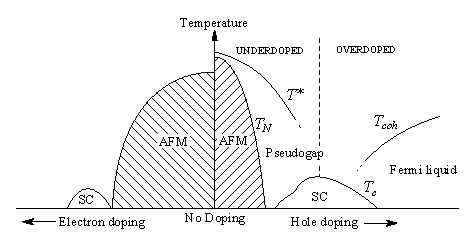
\includegraphics[scale=1.4]{Chapter-Introduction/Figures/ElecHolePhaseDiagram/ElecHolePhaseDiagram}
        \caption{A schematic phase diagram showing electron doped to the left and hole doped to the right. \ac{AFM} is the antiferromagnetic Mott insulating phase, SC is the superconducting phase. $T^*$, $T_N$, $T_c$ and $T_{\textrm{coh}}$ are the temperature scales for the pseudogap, \ac{AFM} state, superconductivity and coherent Fermi liquid phases respectively. Sketch loosely based on ref.~\cite{Orenstein2010}.}
        \label{Fig:Intro:ElecHolePhaseDiagram}
    \end{center}
\end{figure}

\subsection{Mott insulating parent compound}

Starting with the undoped state in figure~\ref{Fig:Intro:ElecHolePhaseDiagram}, the parent compound materials at zero doping are thought to be Mott insulators i.e. the top most filled state on each lattice site contains one electron. In the conventional band picture this should be metallic since the bands are only partially filled, however when we consider a localised picture of electrons where electrons are confined to lattice sites, any movement of an electron to the neighbouring lattice site will cause an energetically costly double occupancy on one site and zero occupancy on another. This causes the electronic \ac{DOS} to become gapped around the Fermi surface and hence suppressed conduction leading to a splitting of the conduction band and an energy gap hence the insulating behaviour.

This is most simply captured in the Hubbard model which encapsulates the charge hopping concept in a two term Hamiltonian. In the `single-band' case\footnote{which actually refers to the fact that each atom has one `orbit' allowing for a maximum occupancy of two electrons~\cite{Tasaki1998}.} one term represents the hopping amplitude, $t$ and another representing the cost for double occupancy, $U$.  

At half filling, the conduction band is split by energy $U$ so that half the states are above the chemical potential and half are below. If the lower of the split conduction band is below a band of another orbital character, a charge insulator state is realised and any hopping of electrons is predominantly between bands of a different orbital character within the same real-space unit cell. Otherwise if the chemical potential lies directly between the split conduction band, a Mott insulating state is realised and electron hopping predominantly occurs between unit cells.

The $t$ term is reduced when the ordering of the sites is antiferromagnetic since for any hopping to occur at all, the spins must be antialigned to avoid double occupancy of like spins. This region dominates the low doping portion of the phase diagram and remains antiferromagnetic until either the temperature is high enough to allow transitions from the Fermi energy to the states at the edge of the gap or the doping has introduced enough double occupancy holes (or electrons) on lattice sites, which can move without the double occupancy energy cost, to overcome the insulating behaviour.

\subsection{Superconducting dome}

With increased doping, the antiferromagnetic state gives way to the superconducting dome at around $p=0.05$ which itself gives way to a Fermi liquid metallic state at a doping of around $p=0.3$. The maximum $T_c$ occurs at around $p=0.16$. Temperature driven transitions from both the antiferromagnetic and the superconducting state are clearly second order thermodynamic phase transitions with jumps in the heat capacity for example, however there are other regions in the phase diagram which are less well defined such as the pseudogap and the Fermi liquid crossover whose temperature scale can depend on the particular probe used and do not have a clear order parameter.

\subsection{Coherent phase}

To the heavily overdoped side of the phase diagram, beyond the superconducting dome lies the coherent region delimited by $T_{\textrm{coh}}$ where the system bears the hallmarks of a `conventional' metal. More specifically this is defined as the region where $\Sigma^{\prime\prime} \propto \omega^2$ which falls in line with Landau Fermi liquid theory, the standard theory used to model conventional metals\footnote{$\Sigma^{\prime\prime}$ is the imaginary part of the self energy which relates to the quasiparticle lifetime (and scattering rate) and $\omega$ is the excitation energy which is related to $T$. For more on Landau Fermi liquids see section~\ref{Sec:Theo:FermiLiquidTheory}.}. This is in contrast to the broadly funnel shaped region above and between $T_{\textrm{coh}}$ and $T^*$ where $\Sigma^{\prime\prime} \propto \omega$ and is sometimes known as the `strange metal' region.

 The implication is that correlations between electrons are sufficiently weak such that the mass enhanced quasiparticles of Landau's Fermi liquid theory are well defined, leading to conventional metal behaviour. A clear indication of this is a dominant $T^2$ term in the resistivity. In the region above $T_{\textrm{coh}}$ we observe an anomalous additional $T$-linear contribution high above the Debye temperature typical for cuprates meaning that it is unlikely to be due to electron-phonon scattering. The confinement of this $T$-linear region to above the superconducting dome has been observed in heavy Fermion materials~\cite{Custers2003} and is often associated with proximity to a \ac{QCP}~\cite{Hussey2008}.

\subsection{The pseudogap}
    \label{Sec:Intro:Pseudogap}

Above the antiferromagnetic region and the superconducting state is one of the most controversial regions of the phase diagram, the so called pseudogap phase. This is a region which was first demonstrated in 1989, just a few years after the discovery of the cuprate materials, by \ac{NMR} measurements performed at Bell labs~\cite{Warren1989}. A noticeable fall in the susceptibility occurs at a temperature significantly above $T_c$ which led to conclusion of possible spin pairing before the onset of bulk superconductivity\footnote{Cooper paired electrons in the singlet state have zero net spin hence they do not contribute to the susceptibility, whereas unpaired electrons do. Cooper pairing leads to a reduction in susceptibility, see for example neutron scattering chapter by S. M. Hayden in ref.~\cite{Hayden}.}. The question arose as to what the exact relation of the pseudogap is to the superconducting state --- is it a precursor state, from which superconductivity arises or is it a competing phase? --- and from a materials development point of view, to obtain higher $T_c$ should we be finding ways to suppress the crossover to the pseudogap state or encourage it?
\begin{figure}[htbp]
    \begin{center}
        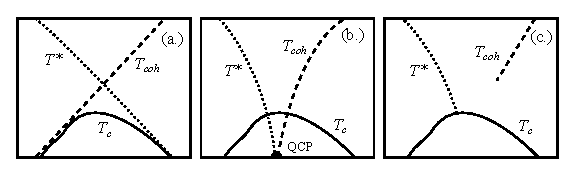
\includegraphics[scale=1.3]{Chapter-Introduction/Figures/PGScenarios/PGScenarios}
        \caption{Three scenarios proposed for the $T^*$ temperature scale behaviour. (a.) the pseudogap as the `precursor' state, (b.) as the `competing' state, (c.) and the `transition' scenario.}
        \label{Fig:Intro:PGScenario}
    \end{center}
\end{figure}
By finding where exactly the $T^*$ energy scale meets the superconducting dome, strong evidence can be found that supports one or the other scenario. However the problem lies in the type of probe used. Select spectroscopic measurements including \ac{STM}, \ac{ARPES} and Raman spectroscopy on materials of comparable $T_c$ values have found that the $T^*$ overreaches the superconducting dome entirely~\cite{Hufner2008}, meeting with the overdoped edge at $T=\unit{0}{\kelvin}$. This supports the precursor state theory illustrated in figure~\ref{Fig:Intro:PGScenario}~(a.) where $T^*$ and $T_{\textrm{coh}}$ cross to define a region which is below both temperature scales where the carrier are both coherent quasiparticles and paired leading to the superconducting condensate.

A second scenario is supported by measurements using bulk probes such as heat capacity, magnetic susceptibility and resistivity measurement have shown the $T^*$ energy scale drops into the top of the superconducting dome~\cite{Tallon2001}. This supports the scenario where the pseudogap is in competition with superconductivity for states at the Fermi surface. Once the pseudogap phase is suppressed, scattering from quantum fluctuations at zero temperature leads to the formation of the superconducting phase at a \ac{QCP} similar to that found in heavy fermion materials. This scenario is supported by the observation of linear scaling of the resistivity with temperature in the region above the superconducting dome which is a hallmark of proximity of a \ac{QCP}.
% Kondo is a competitive scenario which justified based on
% non-monotonicity of coherence as you move from the antinodes on the FS \cite{Kondo2009}

A third scenario is one where the pseudogap simply becomes the superconducting gap as it meets the top of the superconducting dome. However this scenario leaves hanging questions as to the roles of the pseudogap, $T_{\textrm{coh}}$ and other phenomena in the phase diagram which would need to be addressed theoretically. Moreover this picture is rendered less compelling by the observation in \ac{LSCO} of rapidly increasing, low temperature, normal state resistivity inside of the underdoped superconducting dome which implies the non-superconducting energy gap persists into this region.

\subsection{Stripe order Fermi surface reconstruction}
\label{Sec:Intro:StripeOrderReconstruction}

A second contentious region occurs on the underdoped side of the superconducting dome. Stripe order --- i.e. one dimensional charge ordering --- has long been known about in this region in \ac{LSCO}~\cite{Kivelson2003}, however LeBoeuf \etal{} in a recent paper~\cite{LeBoeuf2011} discusses how low temperature Hall data in \ac{Y123} can be interpreted in terms of a Fermi surface reconstruction at $p=0.08$ between two different Fermi surface topologies --- both of which feature stripe order and how stripe order may be more general to the cuprates\footnote{This proposed reconstruction is separate to the more dramatic Fermi surface reconstruction which is thought to occur between the large hole-like Fermi surface on the overdoped side (right panel fig.~\ref{Fig:Intro:LifshitzReconstruction}) and the stripe order phase on the underdoped side (left and centre panel, fig.~\ref{Fig:Intro:LifshitzReconstruction}).}.
\begin{figure}[htbp]
    \begin{center}
        \includegraphics[scale=0.9]{Chapter-Introduction/Figures/LifshitzReconstruction/LifshitzReconstruction}
        \caption{Schematic representation of the reconstruction thought to occur at $p=0.08$. Shaded region are occupied. Adapted from ref.~\cite{Vojta2011}}
        \label{Fig:Intro:LifshitzReconstruction}
    \end{center}
\end{figure}
Figure~\ref{Fig:Intro:LifshitzReconstruction} illustrates the proposed reconstruction where the mobile electron pockets at the top and bottom of the plot at $p > 0.08$ undergo a so called Lifshitz transition and merge into 1D stripes at $p < 0.08$.  Evidence for this is provided in the form of low temperature Hall data where, for $p > 0.08$, $R_H$ is found to drop from positive at high temperatures to negative at low temperatures which is attributed to the formation of the stripe phase with highly mobile electron pockets (hence the negative $R_H$ at low $T$). For $p < 0.08$, $R_H$ still drops but remains positive for all temperatures which the author attributes to a different Fermi surface topology which no longer features the small highly mobile electron pockets. 

However, as we shall see in the next section, an alternative explanation for the low temperature Hall behaviour is suggested based on the anisotropic scattering rate observed in Sr doped \acf{LSCO}.


% the so-called `1/8$^{\textrm{th}}$ anomaly' which corresponds to around 1/8$^{\textrm{th}}$ doping or $p \approx 0.125$. $T_c$ broadly follows an inverse parabola except for a slight depression on the underdoped side illustrated in figure~\ref{Fig:Intro:ElecHolePhaseDiagram}.



\subsection{Previous work by the Bristol group}

Clearly lots of interesting physics is occurring in and around the superconducting dome and a solid understanding of this region is key to understanding the problem of high-$T_c$. Prof. N. Hussey has been involved in many efforts to shed light on the situation and has described how an usual anisotropic scattering term in the resistivity can be explain much of the unusual behaviour in the cuprates~\cite{Hussey2003b, Hussey2011a, Hussey2008}. A summary of the work relevant to this thesis is presented below.

\subsubsection{Links between anisotropic scattering and $T_c$}
    \label{Sec:Intro:AnisotropicScattering}

Simply measuring resistance along different axes gives an averaged scattering rate through all conduction paths and so to build a map of the angle dependent scattering rates, a different technique must be used. In \ac{ADMR}\footnote{Some older literature labels the technique as a measurement of \ac{AMRO}, however \ac{ADMR} is the current preferred term now.} a strong persistent magnetic field is applied before resistance measurements are taken. The field serves two purposes; firstly, to suppress superconductivity so the normal state can be probed, secondly to confine the electrons to orbits perpendicular to the field. By detailed analysis of the change in resistance as the field is applied at various angles, a picture of the angle dependent scattering rate can be determined.

After performing measurements on samples of \ac{TL2201} with dopings ranging from strongly overdoped to slightly underdoped~\cite{Abdel-Jawad2006}, a trend emerged which is illustrated in figure~\ref{Fig:Intro:AnisotropyPhase}. 
\begin{figure}[htbp]
    \begin{center}
        \includegraphics[scale=1.2]{Chapter-Introduction/Figures/AnisotropyPhase/AnisotropyPhase}
        \caption{Schematic of how the scattering rate, $\Gamma$, the Fermi surface, $FS$, and the superconducting gap, $\Delta_g$ evolve with doping across the superconducting dome. Based on figure 1 in ref.~\cite{Taillefer2006}. The dotted line in the scattering is the isotropic part.}
        \label{Fig:Intro:AnisotropyPhase}
    \end{center}
\end{figure}
Here the scattering rate within the $ab$-plane, $\Gamma$, was found to be composed of two terms; an isotropic term which remained constant with doping (dotted circle) and an anisotropic component which scaled with the superconducting gap, $\Delta_g$ (solid line). Moreover it was found that the superconducting gap and the anisotropic scattering rate both shared the same shape, (`d-wave'), and orientation (aligned with the CuO bonds) which suggests that the anisotropic term may be linked with the exotic superconductivity. 

Evidence for the anisotropic scattering term has also been found in \ac{ARPES} measurements. In underdoped samples, Fermi surface spectral weight that coincides with the antinodal points of $\Gamma$ (and $\Delta_G$) disappears~\cite{Norman2010} i.e. coherent particles are lost in the regions of strong scattering.

Further transport measurements which used high magnetic fields to suppress superconductivity and measure resistivity inside the superconductivity dome have also uncovered an unusual $T$-linear term. The measurements showed that the T-linear term did not funnel down to a point (figure~\ref{Fig:Intro:CooperTLinear}) as is typical of \ac{QCP} behaviour in, for example, the heavy Fermion materials~\cite{Custers2003} but instead spread out into the superconducting region in a `foot' shape~\cite{Cooper2009}.
\begin{figure}[htbp]
    \begin{center}
        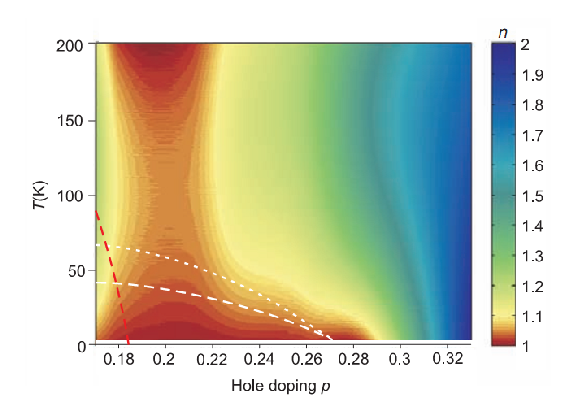
\includegraphics[scale=0.9]{Chapter-Introduction/Figures/CooperTLinear/CooperTLinear}
        \caption{Plot of the $T^n$ term in the fitted field suppressed normal state of Sr doped \ac{LSCO} showing the $T$-linear term extending throughout the superconducting dome and not to a single \ac{QCP}. Taken from Cooper \etal~\cite{Cooper2009}}
        \label{Fig:Intro:CooperTLinear}
    \end{center}
\end{figure}
This behaviour is highly remarkable since it does not follow either of the usual expected \ac{BCS} behaviour (given the `strange metal' scattering dependence) or the expected \ac{QCP} behaviour (since it does not funnel down to a single \ac{QCP} at $T=\unit{0}{\kelvin}$). As of yet, this highly unusual behaviour is still not fully explained and has so far this has only been observed in \ac{LSCO}. \ac{LSCO} is known to be in close proximity to a van-Hove singularity\footnote{A spike in the \ac{DOS} brought about by a flat region of the bandstructure at the Fermi level.} in this region at $p\approx0.18$~\cite{Hashimoto2008} and so it begs the question as to whether this is an effect due to the proximity of the singularity or something more general to the cuprates.


%It changes from a single large hole band of volume $1+p$ to series of small regions of electron and hole Fermi surface of total volume $p$.

\subsubsection{Links between anisotropic scattering and low temperature Hall behaviour}

Narduzzo \etal~\cite{Narduzzo2008} used the anisotropic scattering rate to successfully explain the temperature dependence of the Hall behaviour in Sr doped \ac{LSCO} which did not require the invocation of any Fermi surface reconstruction scenarios as described in section~\ref{Sec:Intro:StripeOrderReconstruction}. Through appropriately curved Fermi surfaces --- described in more detail in section~\ref{Sec:Theo:TopologyEffects} --- the anisotropic scattering can cause $R_H$ to become negative at low $T$ even with an ostensibly large, hole-like Fermi surface similar to that observed in the overdoped regime.

So far, this has only been demonstrated in \ac{LSCO}~\cite{Narduzzo2008} and in order for it to be a viable explanation for the low temperature Hall behaviour in the cuprates, it will need to be demonstrated in other cuprate materials.

% Motivation

% Lograithmic divergence of scattering rate observed in cuprates which
% begins at critical doping and increases as become more underdoped.
% However common factor of cuprates (Y123, Tl2201, LSCO) is a change of
% Fermi surface (in LSCO at least) from hole to electron leading to a
% van Hove singularity(?) which occurs similar to hwere would expect the
% insulating crossover. This does not occur in BSCO however until
% around p=0.2\cite{Hashimoto2008}. If the \alpha^2 term takes off
% earlier for BSCO\cite{Hussey2011a} is good
% evidence that is due to the proximity to van Hove rather  than Moot
% insulator transition.\cite{Ono2000}


% \section{Mott physics}

% The Hubbard model takes the relatively simple and solvable tight-binding model and introduces an Anderson term which raises the energy for double occupancy by an amount $U$, known as the `Hubbard U'. This simple change deeply enriches the physics with one of the outcomes being the existance of the Mott insulating state which occurs when each lattice site is half filled with a single electron. The energy cost for an electron to hop to an adjacent site is so high that it locks the electrons in place, preventing effective conduction. Introducing holes (or electrons) allows once again hopping to take place and the eigenstates are no longer entireley localised.
